\chapter{Thiết kế hệ thống}

\section{Kiến trúc tổng thể}

Hệ thống được tổ chức theo \textbf{kiến trúc ba lớp} trên nền Docker Compose (5 container):

\begin{figure}[h]
\centering
\IfFileExists{figures/deployment.png}{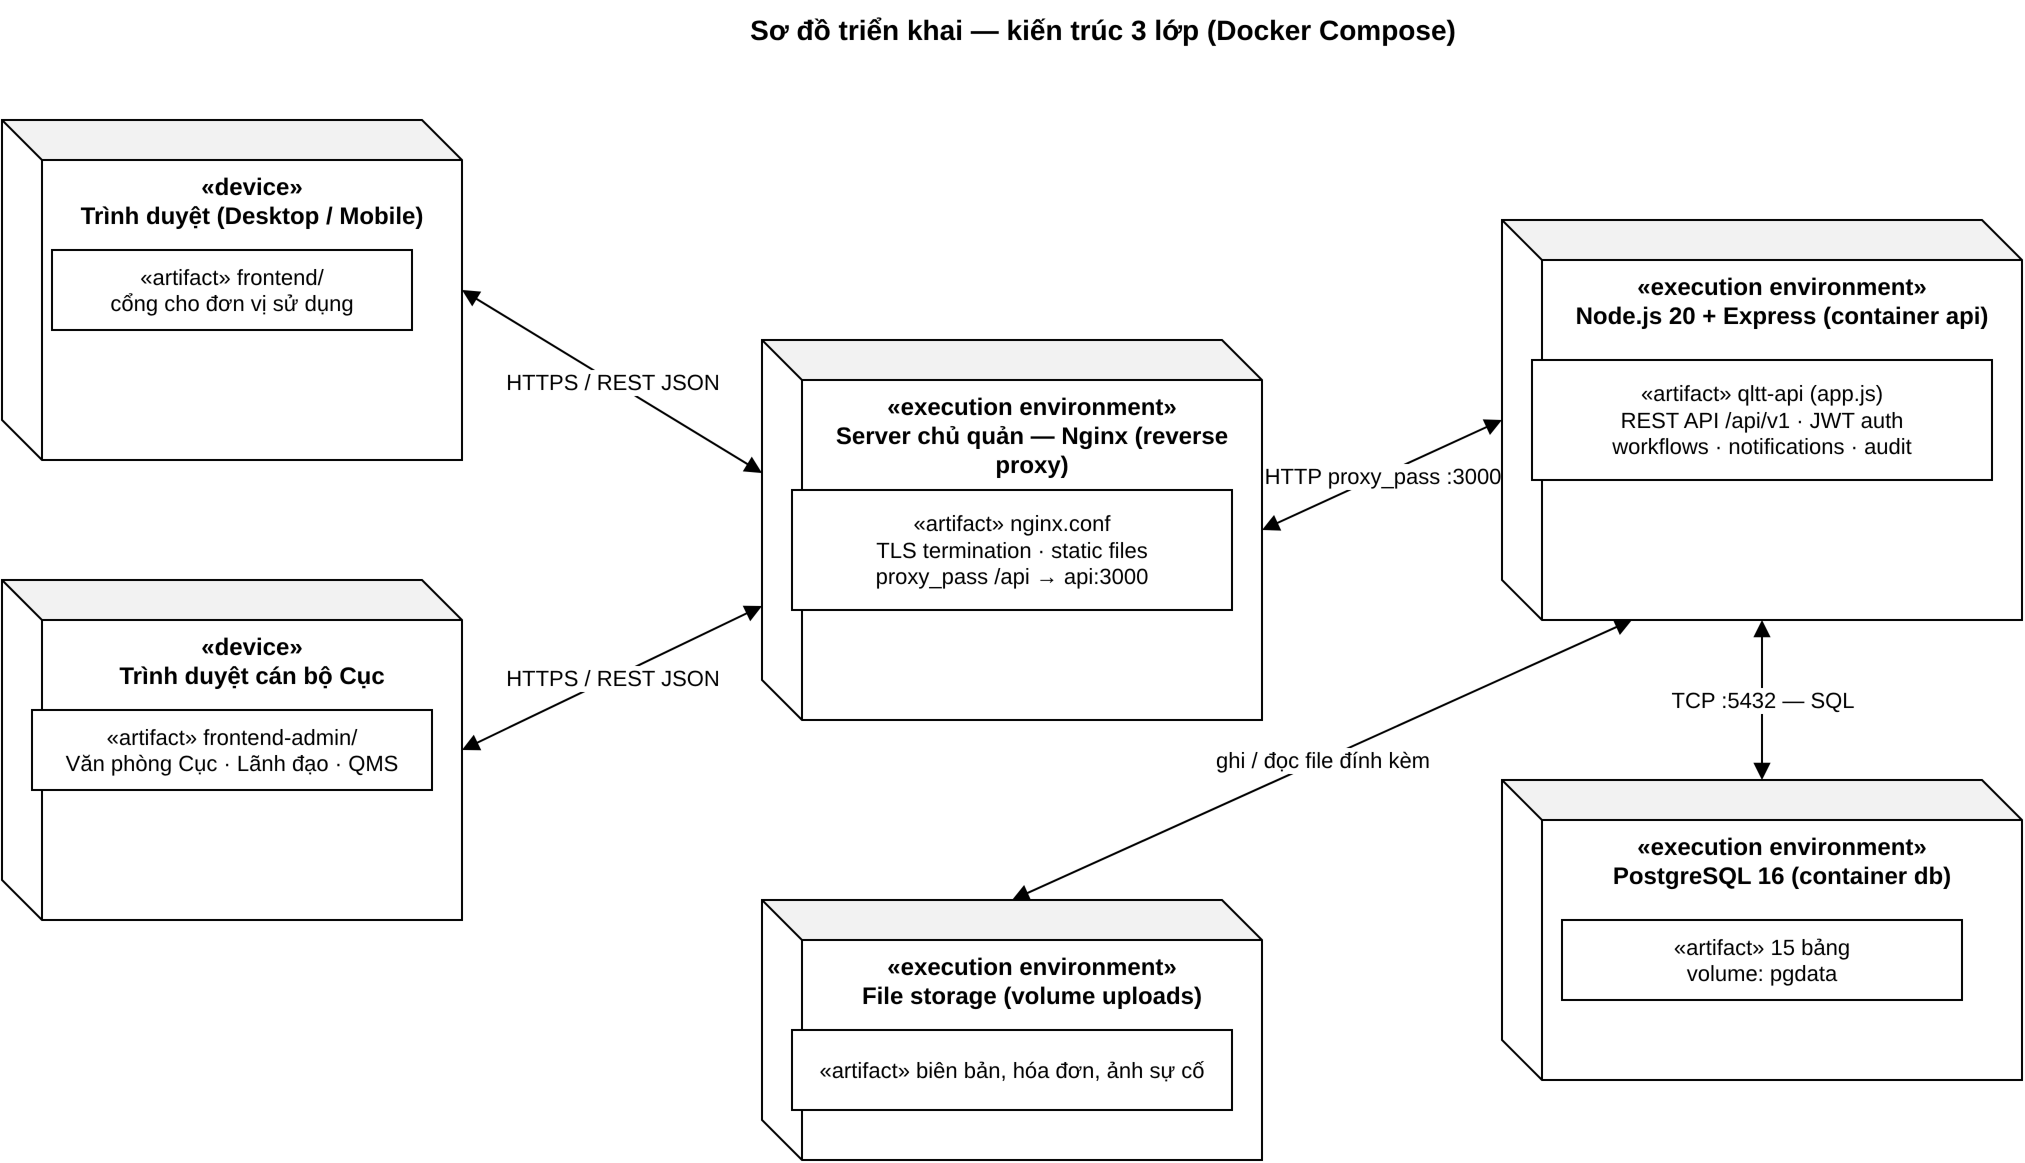
\includegraphics[width=0.96\textwidth]{figures/deployment.png}}{\fbox{\parbox{0.9\textwidth}{\centering Sơ đồ triển khai (file \texttt{docs/diagrams/06-erd-deployment.drawio}, trang 2)}}}
\caption{Sơ đồ triển khai — kiến trúc ba lớp}
\label{fig:deploy}
\end{figure}

\begin{table}[h]
\centering
\caption{Các thành phần triển khai}
\label{tab:components}
\begin{tabular}{P{3.4cm}P{5cm}P{6.6cm}}
\toprule
\textbf{Container} & \textbf{Công nghệ} & \textbf{Vai trò} \\
\midrule
frontend (nginx :8080) & Nginx + HTML/CSS/JS tĩnh & Cổng cho đơn vị sử dụng: tra cứu thiết bị, báo sự cố, theo dõi sự cố, xem kế hoạch \\
frontend-admin (nginx :8081) & Nginx + HTML/CSS/JS tĩnh & Workspace cho Văn phòng Cục / Lãnh đạo Cục / QMS: duyệt, xử lý, báo cáo \\
api (:3001$\rightarrow$3000) & Node.js 20 + Express & REST API \texttt{/api/v1}: nghiệp vụ, state machine phê duyệt, JWT, nhắc lịch (node-cron) \\
db & PostgreSQL 16 & 15 bảng dữ liệu; volume \texttt{pgdata} \\
uploads (volume) & Docker volume & File đính kèm: biên bản, hóa đơn, ảnh sự cố \\
\bottomrule
\end{tabular}
\end{table}

Hai cổng frontend đều proxy \texttt{/api} về container \texttt{api:3000} qua Nginx — trình duyệt chỉ gọi API bằng đường dẫn tương đối, giúp triển khai sau reverse proxy/TLS của server chủ quản mà không cần CORS riêng.

\section{Thiết kế cơ sở dữ liệu}

\begin{figure}[h]
\centering
\IfFileExists{figures/erd.png}{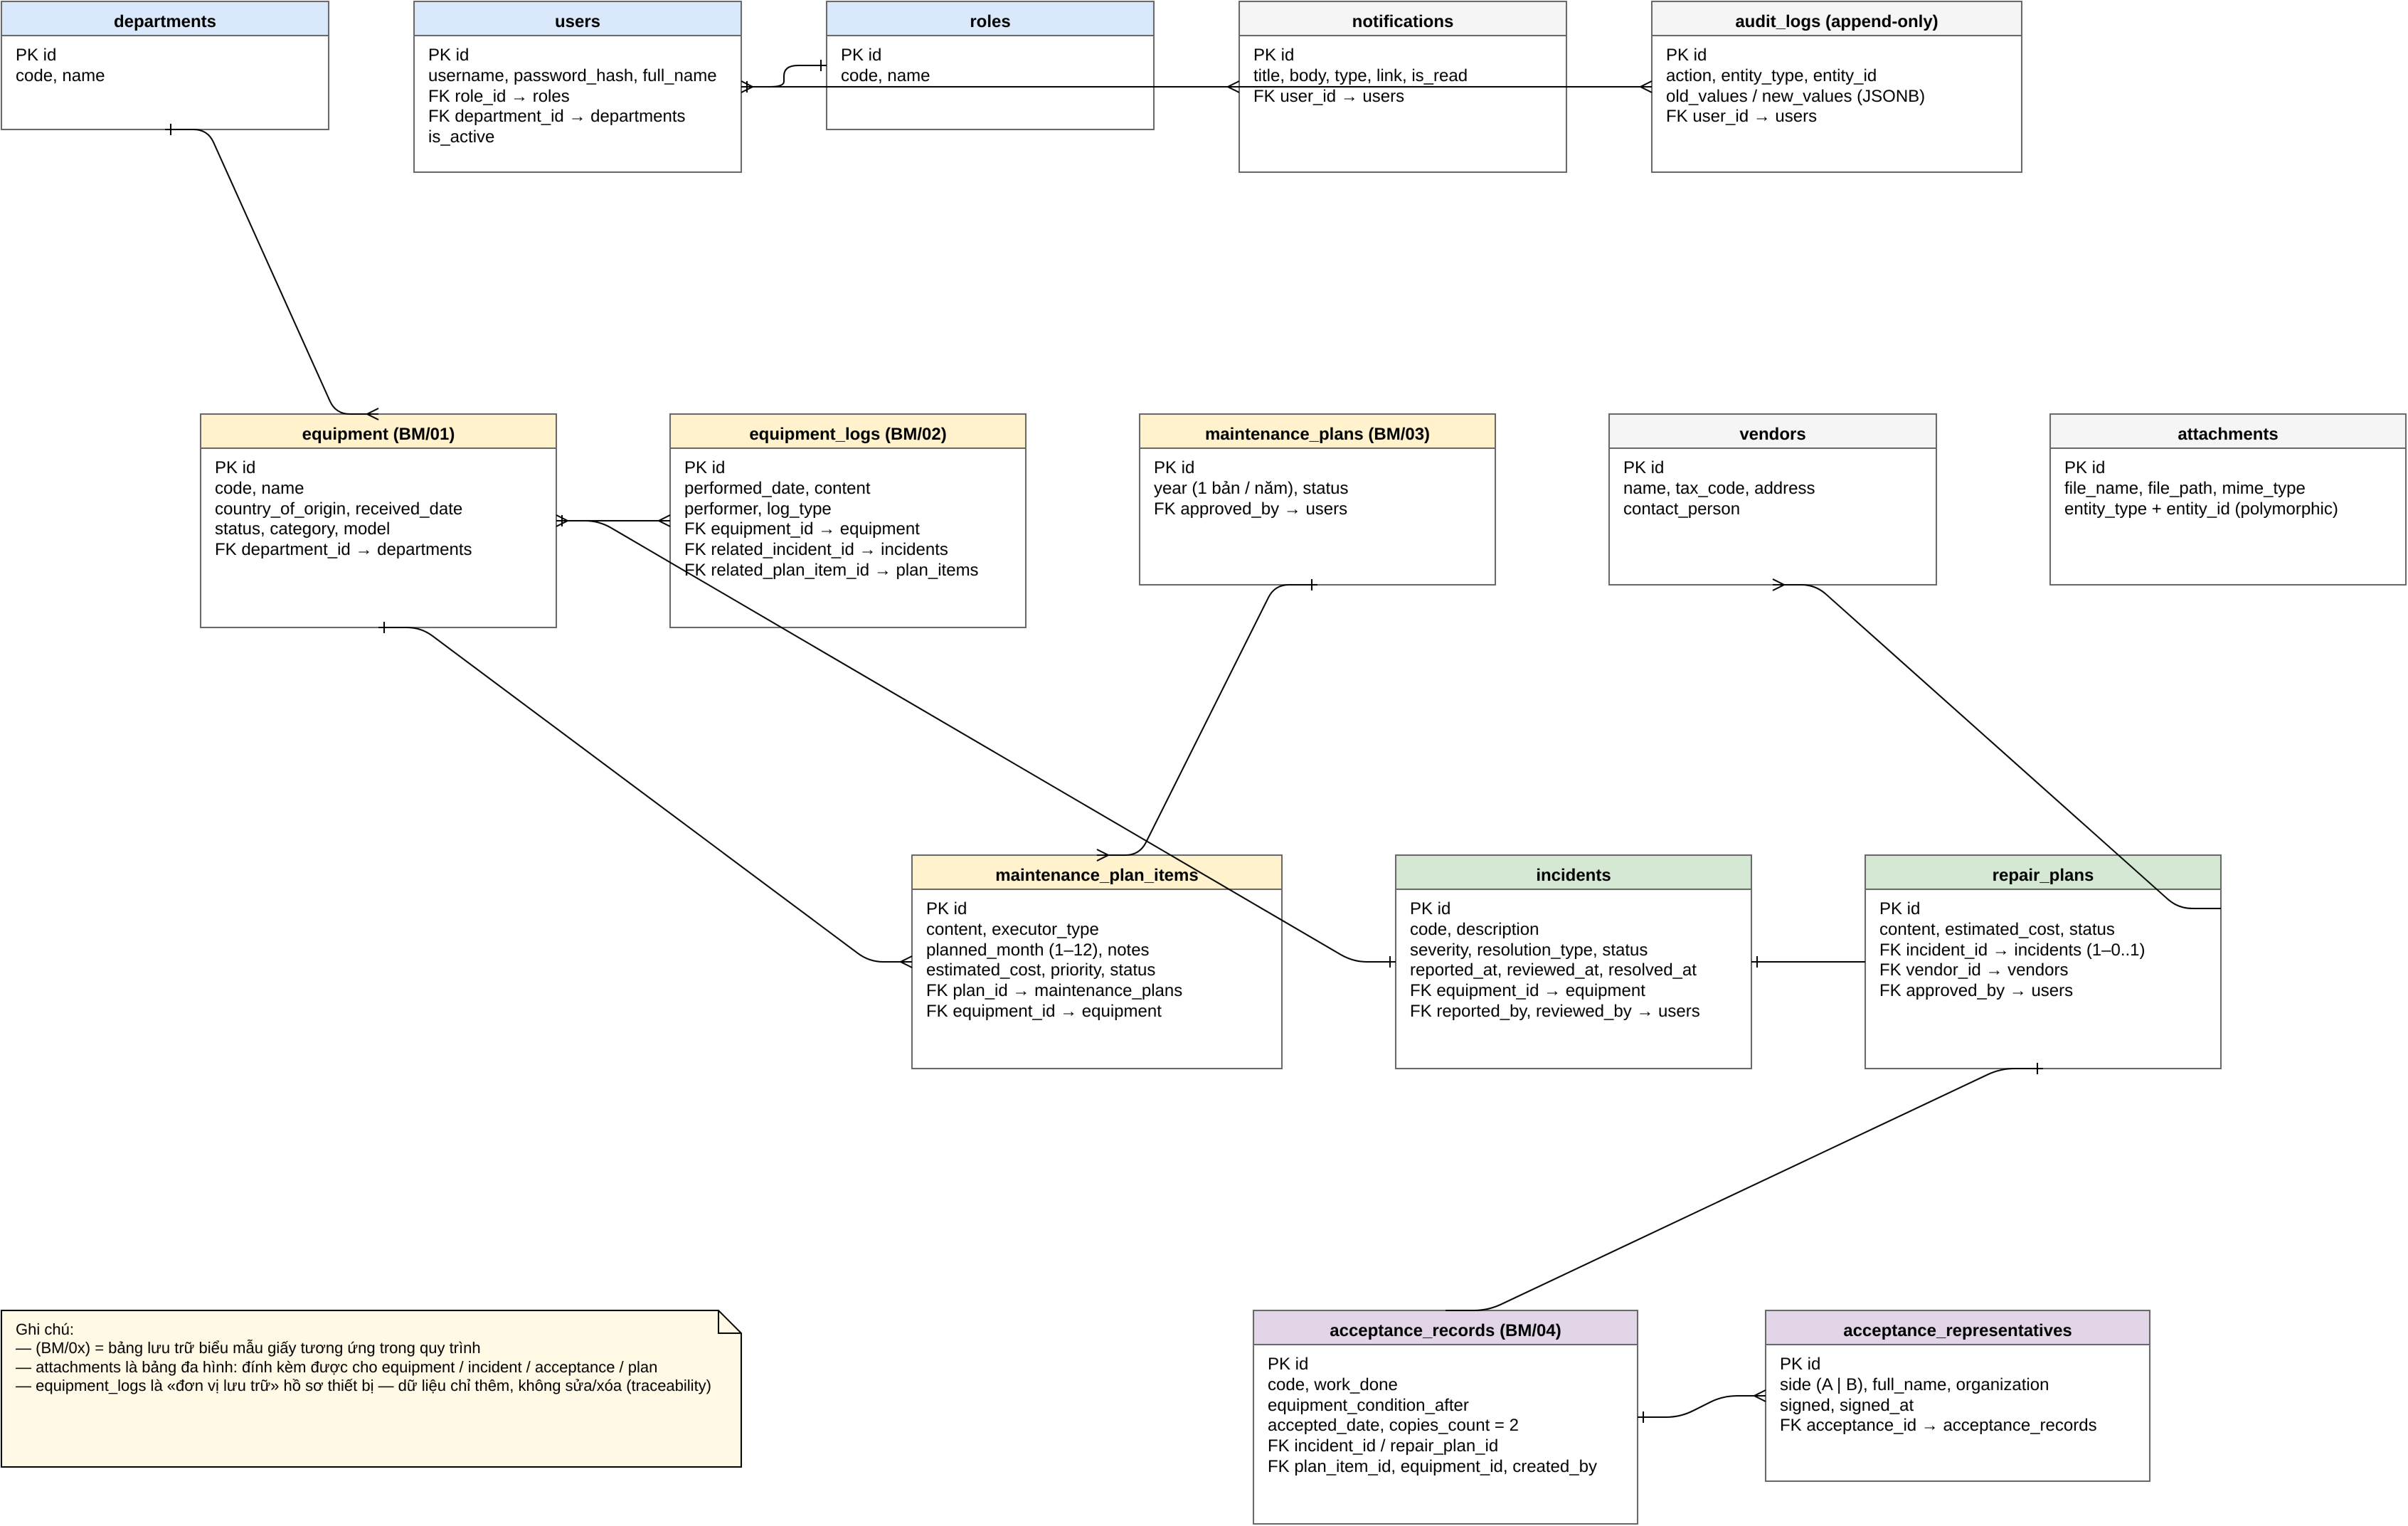
\includegraphics[width=\textwidth]{figures/erd.png}}{\fbox{\parbox{0.9\textwidth}{\centering ERD (file \texttt{docs/diagrams/06-erd-deployment.drawio}, trang 1)}}}
\caption{Sơ đồ thực thể — quan hệ (ERD) của cơ sở dữ liệu}
\label{fig:erd}
\end{figure}

Lược đồ gồm 15 bảng: \texttt{departments, roles, users, equipment, equipment\_logs, maintenance\_plans, maintenance\_plan\_items, incidents, repair\_plans, vendors, acceptance\_records, acceptance\_representatives, attachments, notifications, audit\_logs}. Các bảng cốt lõi:

\begin{longtable}{P{3.6cm}P{4.6cm}P{3cm}P{3.6cm}}
\caption{Lược đồ các bảng chính (nguồn gốc trường ghi trong ngoặc)}\label{tab:schema}\\
\toprule
\textbf{Bảng} & \textbf{Trường chính} & \textbf{Khóa ngoại} & \textbf{Nguồn gốc} \\
\midrule
\endfirsthead
\toprule
\textbf{Bảng} & \textbf{Trường chính} & \textbf{FK} & \textbf{Nguồn gốc} \\
\midrule
\endhead
equipment & code (Mã số), name (Tên), country\_of\_origin (Nước SX), received\_date (Ngày nhận), status [mở rộng] & department\_id & BM/01 \\
\addlinespace
equipment\_logs & performed\_date (Ngày thực hiện), content (Nội dung), performer (Người thực hiện), log\_type [mở rộng] & equipment\_id; related\_incident\_id; related\_plan\_item\_id & BM/02 \\
\addlinespace
maintenance\_plans & year (Năm, duy nhất), status, approved\_by, approval\_note & created\_by & BM/03 (header) \\
\addlinespace
maintenance\_plan\_items & content (Nội dung), executor\_type (nội bộ/bên ngoài), planned\_month (tháng), notes (Ghi chú); estimated\_cost, priority [mở rộng] & plan\_id; equipment\_id; department\_id & BM/03 (dòng) \\
\addlinespace
incidents & code [mở rộng], description, severity [mở rộng], resolution\_type, status, reported\_at & equipment\_id; reported\_by; reviewed\_by; department\_id & 6.2.3b \\
\addlinespace
repair\_plans & content, estimated\_cost [mở rộng], status phê duyệt & incident\_id (1--0..1); vendor\_id & 6.2.3b \\
\addlinespace
acceptance\_records & code, work\_done (đã thực hiện), equipment\_condition\_after (tình trạng sau), accepted\_date, copies\_count = 2 & incident\_id; repair\_plan\_id; plan\_item\_id; equipment\_id & BM/04 \\
\addlinespace
acceptance\_representatives & side (A/B), full\_name (Ông/bà), organization (Đơn vị), signed & acceptance\_id (hợp thành, CASCADE) & BM/04 \\
\addlinespace
audit\_logs & action, entity\_type, entity\_id, old\_values/new\_values (JSONB) & user\_id & ISO 9001 \\
\bottomrule
\end{longtable}

\textbf{Quy tắc thiết kế quan trọng:}
\begin{itemize}
  \item \texttt{equipment\_logs} và \texttt{audit\_logs} là hai bảng \emph{append-only}: ứng dụng không cung cấp UPDATE/DELETE — bảo đảm truy vết theo ISO 9001:2015.
  \item Trạng thái (status) được mã hóa bằng hằng số chuỗi có kiểm soát ở tầng API (state machine), không cho phép nhảy trạng thái tùy ý.
  \item \texttt{attachments} là bảng đa hình (entity\_type + entity\_id) — một cơ chế cho mọi loại đối tượng.
  \item Kế thừa TaiLieu được phẳng hóa (mục 4.4); hợp thành dựng bằng \texttt{ON DELETE CASCADE}.
\end{itemize}

\section{Thiết kế giao diện}

Hệ thống có \textbf{hai cổng} tách bạch theo đối tượng người dùng:

\begin{itemize}
  \item \textbf{Cổng đơn vị sử dụng} (theme tối, gold): trang chủ giới thiệu nghiệp vụ; tra cứu danh mục (đúng 6 cột BM/01); hồ sơ thiết bị dạng timeline (BM/02); form báo sự cố tối giản cho mobile; theo dõi sự cố của đơn vị với nút ``Tự khắc phục''; xem kế hoạch năm theo tab năm.
  \item \textbf{Cổng quản trị} (theme sáng, pastel): dashboard tổng quan với 4 thẻ số liệu thật và biểu đồ sự cố 12 tháng; bảng danh mục thiết bị + modal thêm/sửa + xuất Excel; xử lý sự cố (xem xét/phân loại, lập phương án); phương án sửa chữa (duyệt/từ chối/hoàn thành theo vai trò); kế hoạch năm (tạo nhiều hạng mục, trình duyệt, cập nhật tiến độ); nghiệm thu (lập biên bản với đại diện hai bên, ký); nhà thầu; người dùng \& phân quyền; báo cáo thống kê; nhật ký thao tác.
\end{itemize}

Nguyên tắc thiết kế: (i) bảng hiển thị \emph{giữ nguyên các cột của biểu mẫu giấy} để người dùng chuyển tiếp dễ; (ii) nút hành động chỉ hiện khi vai trò và trạng thái cho phép (UI phản ánh đúng state machine); (iii) responsive mobile-first cho luồng báo sự cố.

\section{Thiết kế bảo mật và kiểm soát tài liệu}

\begin{table}[h]
\centering
\caption{Ma trận phân quyền theo vai trò (tầng API)}
\label{tab:roles}
\begin{tabular}{P{4.4cm}P{10.6cm}}
\toprule
\textbf{Vai trò} & \textbf{Quyền} \\
\midrule
Đơn vị sử dụng & Xem thiết bị/hồ sơ của đơn vị mình; báo sự cố; tự khắc phục; cập nhật tiến độ hạng mục; ký biên bản (nếu là đại diện) \\
Văn phòng Cục & Toàn bộ CRUD danh mục/hồ sơ; xem xét sự cố; lập phương án/kế hoạch/biên bản; quản trị người dùng, nhà thầu; xuất Excel; xem nhật ký \\
Lãnh đạo Cục & Phê duyệt/từ chối kế hoạch và phương án; ký nghiệm thu; xem báo cáo \\
Ban QMS & Xem toàn bộ + báo cáo + nhật ký thao tác (không sửa nghiệp vụ) \\
Nhà thầu & Xem phương án liên quan; ký nghiệm thu (mở rộng) \\
\bottomrule
\end{tabular}
\end{table}

Cơ chế kỹ thuật: mật khẩu băm \texttt{bcrypt}; phiên \texttt{JWT} 8 giờ; middleware \texttt{authenticate} + \texttt{requireRole} chặn từng endpoint; middleware \texttt{attachAudit} ghi mọi thao tác quan trọng (CREATE/UPDATE/APPROVE/REJECT/SUBMIT/SIGN/LOGIN...) vào \texttt{audit\_logs} kèm dữ liệu cũ/mới dạng JSONB; file tải lên giới hạn 20MB, tải xuống qua route có xác thực.

\section{Thiết kế nhắc lịch và thông báo}

Job \texttt{node-cron} chạy \texttt{0 7 * * *}: truy vấn các hạng mục của kế hoạch \emph{đã duyệt} có tháng dự kiến trùng tháng hiện tại mà chưa hoàn thành $\rightarrow$ gửi thông báo cho Văn phòng Cục và các thành viên của đơn vị sử dụng liên quan. Thông báo trong hệ thống (\texttt{notifications}) đánh dấu đọc từng người dùng; chấm đỏ trên topbar phản ánh số chưa đọc.

\section{Thiết kế workflow (state machine trong mã nguồn)}

Thay vì BPM engine nặng, nhóm dùng state machine đơn giản: mỗi bản ghi có cột \texttt{status}; mỗi transition được cài đặt trong handler có kiểm tra trạng thái hiện tại (UPDATE ... WHERE status = ... RETURNING) — nếu không khớp trả 409. Điều này bảo đảm:
\begin{itemize}
  \item không thể duyệt một kế hoạch chưa trình, không thể ký biên bản đã ký;
  \item nhánh ``sự cố nhỏ'' được tối ưu: \texttt{review(TU\_KHAC\_PHUC)} $\rightarrow$ \texttt{self-resolve} $\rightarrow$ đóng, chỉ hai bước;
  \item mọi chuyển trạng thái đều phát sinh thông báo + audit log.
\end{itemize}
